In this chapter we will describe the architecture of the entire system by first showing the overall structure followed by a short description of the individual components.
The platform allows lecturers to create a syllabus that includes problem sets, exercises and test cases for the exercises. Additionally, students can do the exercises that the lecturer has provided.
The platform is a web application designed using a client-server architecture. Using this architecture the client communicates with a server using HTTP to send \textit{request} messages. The server waits for client requests and processes the requests when they arrive and replies to the requests with a \textit{response} message.

The platform has a user-interface as well as business logic to handle user requests. The platform supports role-based authentication with roles, meaning that users of varying roles have access to different functionality. The platform can run tests, to check whether a piece of code solves an exercise. Account data, test runs, and syllabus data is persisted in a database.
The overall architecture for the system can be seen in figure \ref{fig:Architecture}.

\begin{figure}[H]
	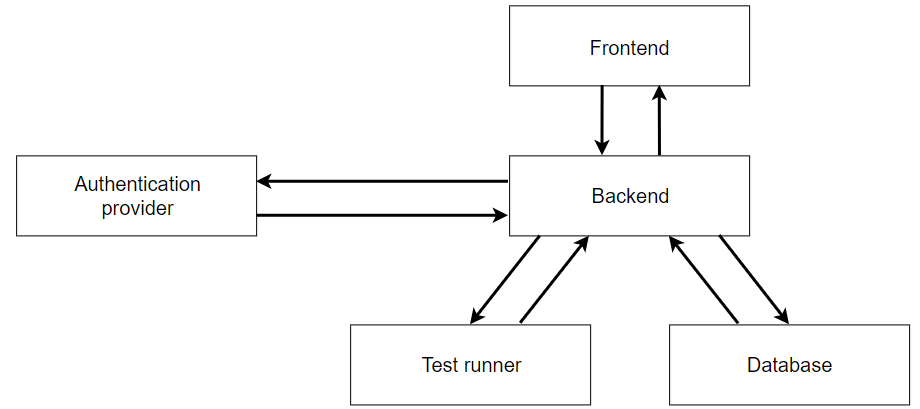
\includegraphics[scale=0.6]{Architecture.PNG}
	\centering
	\caption{The architecture for our web application}
	\label{fig:Architecture}
\end{figure}

Note that the platform has an API running on a separate server instance to handle code execution and test, called \textit{Test Runner}. As components are introduced in the following sections, we elaborate on the choices made for each component, in relation to this structure.

\section{Back-end system}
The back-end system has several responsibilities including routing, data retrieval and updates and orchestration of execution of code tests. The backend is the link between all the components in the system. It operates as a traditional server in a client-server architecture.

\section{Frontend}
The frontend is the user facing component of our web application. The frontend is designed such that its user-interface and functionality is dependent on the role of the user.
For example if a student has signed in, the student is able to see and complete exercises. In turn if a lecturer signs in, they will have access to more functionality such as creating a syllabus or exercise.

Regardless of the roles of the user the frontend has the ability to send data to the backend for storage, and show the output of executed code, by sending it to the backend and showing the response.

\section{Database}
In order persist data, the backend retrieves and updates data in the database component depicted in figure \ref{fig:Architecture}. This is done through create, read, update and delete operations.
The backend then queries the database and returns the relevant data.

The database component is implemented as a Postgres database. The entities and their relationships contained within the database is shown in figure \ref{fig:Database}. In the figure each box represents an entity-set and attributes for the entities. A diamond represent a relationship between two or more entity-sets.

A dotted line connecting an entity-set to a relationship represent a partial participation of the connected entities and the other participants in the relationship. This means that an entity can exist in the database without participating in the relationship.
A full line connecting an entity-set to a relationship represents total participation of the entity-set symbolizing that an entity must participate in the relationship.
This means that an entity cannot exist in the database without participating in the relationship.
The numbers and letters at the beginning of each relationship line represents the cardinality. A \textit{number} between a relationship and an entity-set represents the number of times an entity can participate in the relationship. Similarly, an \textit{N} represents that entities can participate $0$ or more times.

\begin{figure}[H]
	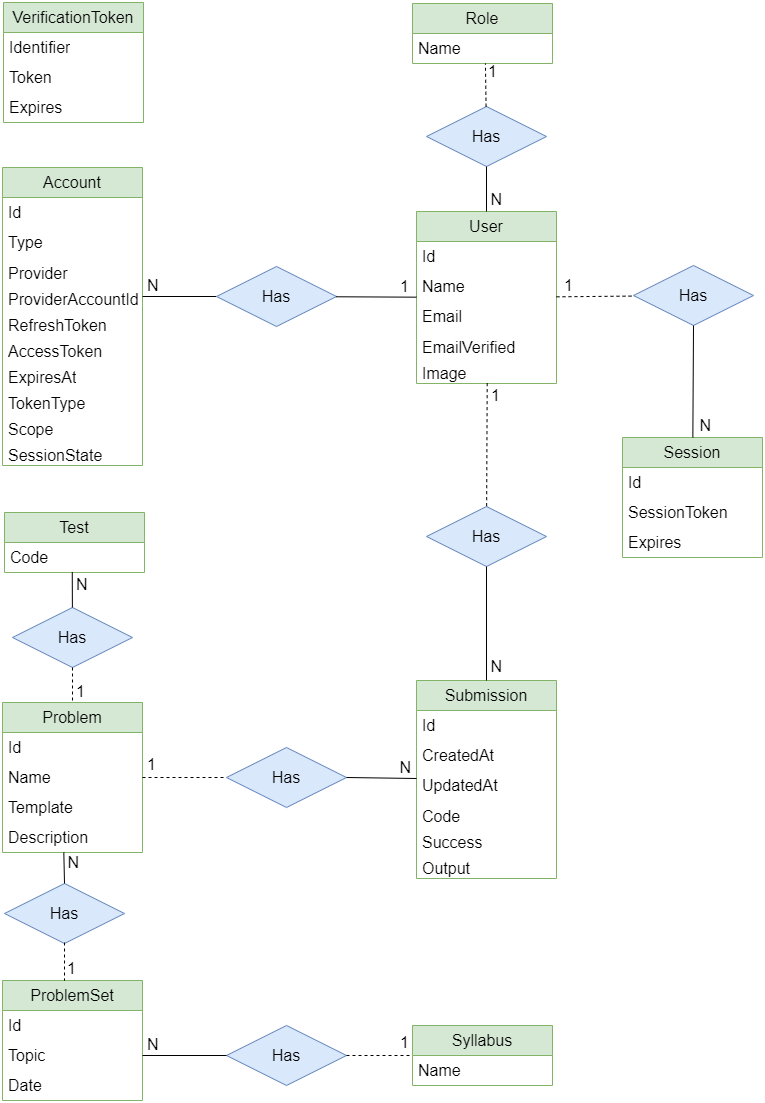
\includegraphics[scale=0.4]{Database.png}
	\centering
	\caption{Entity relationship diagram of the database}
	\label{fig:Database}
\end{figure}

The structure of database can be explained through the two types of users of the system. The lecturer and the student.
In order to support different roles in the system, we have created the entities \textit{Role} and \textit{User}. The \textit{Role} entity has one attribute called \textbf{Name}. This corresponds to the name of the role. The \textit{User} entity has the attributes \textbf{Id}, which is a unique identifier, \textbf{Name}, \textbf{Email}, \textbf{EmailVerifed} which is when the email was verified and an \textbf{Image} attribute which contains the URL for an image of the user. The \textit{User} entity has a many-to-one relationship with the entity \textit{Role}, which means that users can only have one role.

To support a lecturer in creating a syllabus for a semester course we have created the entities \textit{Syllabus}, \textit{Problemset}, \textit{Problem} and \textit{test}. For each entity, a set of attributes have been added to contain the relevant data and relationships between these entities to annotate their relation.
For the \textit{Problem} entity we have added an \textbf{Id} attribute as a unique identifier, a \textbf{Name} attribute, a \textbf{Template} attribute, which contains code that will be automatically included in the editor when starting a problem. This ensures that the functions are included in a module which can later be accessed by \textbf{Hspec}. The final attribute is the \textbf{Description}, which contains the description of the exercise.

The \textit{Test} entity has the attribute \textbf{Code}. This contains the test code that the lecturer has written for a problem. A \textit{Problem} and a \textit{Test} are in a one-to-many relationship with each other, where a \textit{Problem} has many \textit{tests}. This allows a lecturer to define multiple tests for a problem.

The \textit{Problemset} entity corresponds to a course exercise session. It has the attribute \textbf{Id}, which a unique identifier, the attribute \textbf{Topic} which is the topic covered in the session, and lastly a \textbf{Date} which corresponds the when the session occurs. The relationship between the \textit{Problemset} entity and the \textit{Problem} entity is one-to-many, since a problem set has multiple problems. This allows the lecturer to create a set of problems for a course exercise session.

The \textit{Syllabus} entity corresponds to an entire syllabus for a course. The entity only has a \textbf{Name} attribute, which is the name of the course. The \textit{Syllabus} entity has a one-to-many relationship with the \textit{Problemset} entity. This allows the lecturer to create multiple problem sets for a course.

To support a student in submitting solutions to exercises we have created the entity \textit{Submission}. This entity contains the attributes \textbf{Id}, which is a unique identifier, \textbf{CreatedAt} which contains the time for when the submission was first added, \textbf{UpdatedAt} which contains the time when the submission was last updated. It also contains the attributes \textbf{Code}, which contains the code submitted by the student, \textbf{Success} which states whether the submission passed the tests for the problem. Finally it has the attribute \textbf{Output}, which is the standard output from the compiler.
The \textit{Submission} entity is in a many-to-one relationship with the \textit{User} entity, because each user can have many submissions. \textit{Submission} is also in a many-to-one relationship with \textit{Problem}, as a problem can have multiple submissions.

The remaining entities \textit{Account}, \textit{Session} and \textit{VerificationToken} are entities which are required by authentication services and are not developed by us.

\section{Test Runner}
As previously mentioned, the platform is able execute code by sending the submitted code to the Test Runner API which verifies whether the code is syntactically correct and satisfies the tests defined by the lecturer.
Since the Test Runner is running on its own server instance, we created endpoints that allow the backend to communicate with the Test Runner API. When the submitted code has been processed the output will be returned to the caller.

In the following chapters we will elaborate on the most important components of our system. In these chapters we will give a detailed description of how the components work and their structure.